\section{Clouds role in the climate system} \label{sec:cloud_in_climate_system}
% Clouds, climate and machine learning
Clouds play an important role in the climate system. Both affecting the radiative budget and the hydrological cycle. Understanding how clouds form in the complex system of the atmosphere involves both knowledge about the large scale influence by the circulation and the small scale influenced by aerosols. Clouds are composed of liquid droplets, ice crystal or both. To this day the micro-physics of all phases are not fully understood. Here mixed phase clouds, consisting of both liquid and ice, shows to be the most difficult. 
%Climate models are the most useful tool for studying the past, present and future climate. Clouds and aerosols are acknowledged as the factors contributing with the largest uncertainty to the \acrfull{ecs}. Also known as global mean temperature increase as a consequence of doubling of the pre-industrial levels of $CO_2$ (280 \acrshort{ppm}). \textbf{kilde AR4 which ch?} \textit{It remains unclear to which level of sophistication is adequate to model their effect om climate.} (\cite{IPCC_CH7_clouds}).

%\textbf{Make sure you include everything that's related to parametrised processes.}
It is understood that cloud formation requires suitable aerosols and sufficient supersaturation. \textit{Aerosols} include both gases and solid particles suspended in air. They interact with the clouds by serving as particles which vapour and ice can condensate or deposit upon. The different phases require different properties and the nuclei are called \acrfull{ccn} for liquid droplets and \acrfull{inp} for ice crystals. Saturation is usually achieved by a temperature decrease in rising air masses. %Thus the stability of the atmosphere  plays a key role for convective motions.
%\textbf{Legg inn bilde a skyer en i is fase og en i liquids. Skriv noe som "the sharp outoline suggest that the cloud is consisting of liquid droplets, even at temperagtures below 0."}
%The negative temperature decreases by height is often referred to as the lapse rate, $\Gamma_{s, d}$. 
 
Growth processes are phase dependant. Liquid droplet grows by diffusion and later by collision and coalescence. At temperatures around -38 $^oC$ (\cite{lohmann2016}) droplets spontaneously freeze and can act as \acrshort{inp}. Clouds consisting purely of ice crystals first grow by deposition of vapour then by aggregation (\cite{Fowler1996LiquidAssumptions}). In the presence of both phases, droplets evaporate and deposit on to the ice crystals.
%When both phases are present in a cloud, the saturation vapour pressure over ice is higher than over liquid. This may cause the droplets to evaporate and deposit on to the ice crystals. 
This mechanism exist because the saturation vapour pressure, $e_s$ is lower with respect to ice than water. It is most efficient at 12$^oC$ when the difference is largest. This is called the Wegeron-Bergeron-Findeisen process.

The equilibrium saturation vapour pressure, $e_s$ is the amount of vapour the air can retain at a given temperature. Its relationship to temperature, $T$ is described by the Clausius-Claperon Equation \eqref{eq:clausius-claperon}, here $L_v$ is latent heat of phase transition vapour in $J g^{-1}$, $M_w$ is and $R^*$ is .
\begin{equation} \label{eq:clasius_claperon}
    \frac{1}{e_s} \frac{de_s}{dT} \simeq \frac{L_v}{R_v T^2} = \frac{L_v M_w}{1000R^*T^2}
\end{equation}
\begin{equation} \label{eq:clasius_claperon_prop}
     \frac{de_s}{e_s} \propto \frac{dT}{T^2} 
\end{equation}
From Equation \eqref{eq:clausius-claperon} it becomes clear that the  is inversely proportional with the second power of the temperature, meaning that for decreasing temperatures the vapour pressure 

Double check if this id only valid for adiabatic processes, is there any other assumptions..?

$R^*$ is the specific gas constant 共the universal
gas constant divided by the mean atmospheric molecular
weight. 
\section{Clouds in the current climate} \label{sec:intro_cloud_current_climate}
\begin{figure}[h]
    \centering
    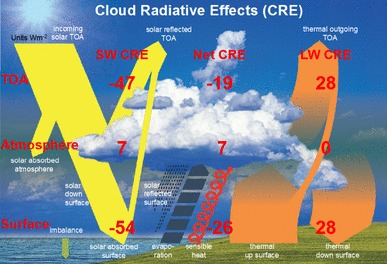
\includegraphics[scale = 7]{Chapter1_Intro/images/CRE_wild2019.jpg}
    \caption{Cloud radiative effect, CRE is the difference between the radiative components of the Clear sky radiative and the all sky. Modified version of as Figure 15 in \cite{Wild2019TheModels}. \textbf{pappa syns denne var grusomt vanskelig.}}
    \label{fig:cre}
\end{figure}
Based on remote sensed and in-situ measurements \citeauthor{Wild2019TheModels} have quantified the contribution of elements in the radiative budget (see Figure \ref{fig:cre}). Cloud radiative effect (\acrshort{cre}) in earth annual mean energy budget is the difference between a cloudy and a cloud-free atmosphere. 

\textbf{Write short paragraph on the components of the energy balance}

The physical properties causing the interaction with radiation is described below. Dense low level clouds reflect solar radiation. This is called the albedo effect. \textit{Albedo} being the ratio between reflected to incoming radiation. The higher number concentrations of droplets in a cloud the higher the total surface area of droplets. The more radiation gets reflected back into space. Clouds absorb longwave radiation and re-emits it. 
\begin{equation} \label{eq:stefan-boltzmann}
    F = \sigma \epsilon T ^4
\end{equation}
The absorbed radiation originates from the surface and is given by Stefan-Boltzmann forth-power law, see equation (\ref{eq:stefan-boltzmann}). The emissivity, $\epsilon$ depends on the (composition, compactness and surface roughness) of the medium. Water, snow and ice have different spectral emissivity (\cite{Huang2018ImprovedClimate}). Different parts of the globe are covered by different surfaces and \citeauthor{Huang2016AnSimulations} proved that assuming a constant surface emissivity effects the \acrfull{toa} polar energy budget \textbf{read paper again to detemine why this is of importance}. The greenhouse effect increases with the cloud altitude, since the temperature difference between the surface and cloud increase. High clouds with low temperatures and  re-emitted radiation at a lower intensity than they absorbed. Researchers are still working on determine the emissivity of the different phases. Despite the uncertainties related to emissivity of the medium, the re-emitted radiation is of a lower intensity than what it absorb.

%This is shown in equations \eqref{eq:cre_sw} and \eqref{eq:cre_lw}. \textbf{drop equations..?}


As shown in Figure \ref{fig:cre} \citeauthor{Wild2019TheModels} concludes with a reduction in shortwave radiation of $-47Wm^{-2}$ by clouds. In other words clouds reflect approximately 50\% of the incoming solar radiation. The clouds are resposible for emmitting $28Wm^{-2}$ in the long wave spectrum. This gives a net \acrshort{cre} of $-19Wm^{-2}$. Proving that the net effects of clouds on the radiative budget is negative.The altitude along with the composition determines the radiative properties of the cloud. 


%\begin{equation} \label{eq:cre_sw}
%    CRE_{sw} = SW\uparrow_{clear-sky} - SW\uparrow_{all-sky}
%\end{equation}
%\begin{equation} \label{eq:cre_lw}
%    CRE_{lw} = LW\uparrow_{clear-sky} - LW\uparrow_{all-sky}
%\end{equation}


\section{Clouds in future climates} \label{sec:intro_cloud_future_climates}
\begin{figure}[h]
    \centering
    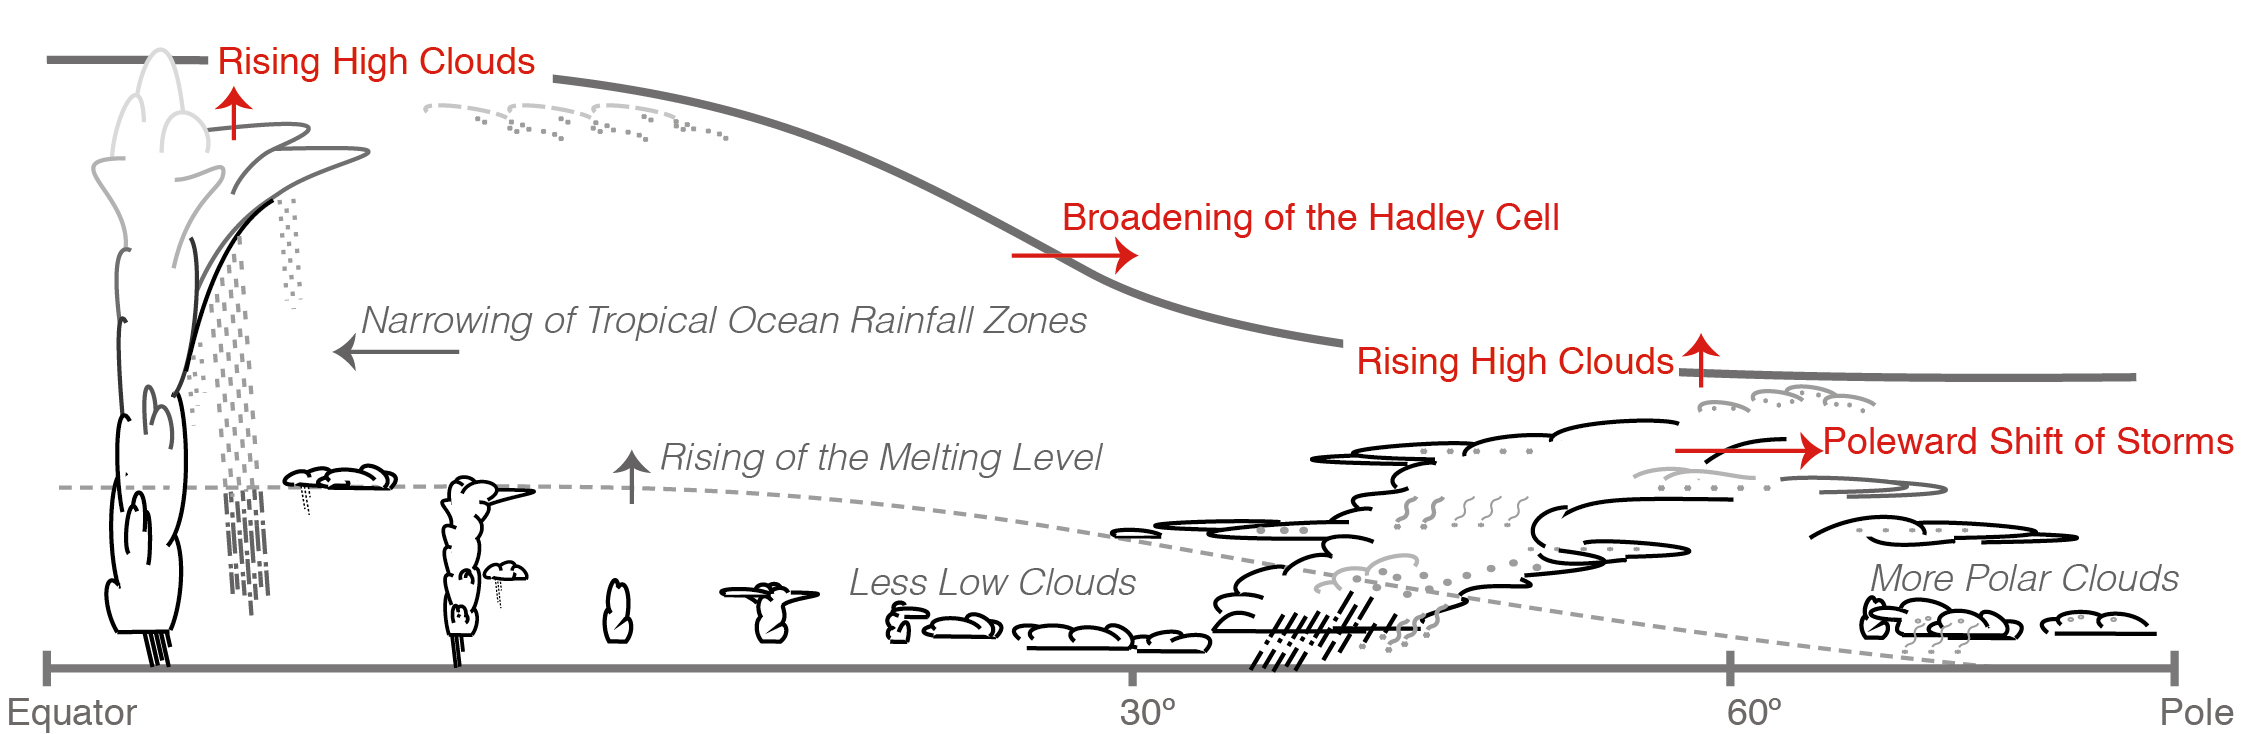
\includegraphics[scale = 0.8]{Chapter1_Intro/images/Fig7-11_ipcc.jpg}
    \caption{Cloud climatology in future climate. Developed based feedback's in climate models, the different adjustments have different uncertainty (\cite{IPCC_CH7_clouds}).}
    \label{fig:cloud_scheme}
\end{figure}
As concluded in the previos section, an excess of radiation gets trapped in the earth system, forcing the surface temperature to increase in order to close the radiative budget. The imbalance at the \acrshort{toa} is estimated by \citeauthor{Wild2019TheModels} to be $0.6W m^{-2}$. 
% Wild et. al. 2019  \textbf{siter} finds an imbalance of This heat gets trapped in the earth system, forcing the surface temperature to increase in order to close the radiative budget. 
%The imbalance in the radiative budget at \acrfull{toa} is the radiative forcing. 
Climate drivers include both natural and anthropogenic forcings. A \textit{forcings} can be everything from natural variability in the solar energy output, volcanic eruptions or greenhouse gas emissions. The climate science community works toward a common goal to determine the \acrshort{ecs} as a function of forcing. Different emission scenarios result different \acrshort{ecs}. The temperature increase induces climate changes. The \acrshort{ipcc} (\cite{IPCC_CH7_clouds}) suggest the following shift in cloud schemes (see Figure \ref{fig:cloud_scheme}). Figure \ref{fig:cloud_scheme} shows a summary of the most likely cloud feedback's. First, a broadening of the Hadley cell causes a poleward shift of storms. This dries up the subtropics and moistens the higher latitudes. Due to the spherical geometry of the Earth, the solar radiation available for reflection decrease poleward. %proportional with the $sin\left(\theta \right)$, where $\theta$ describes the latitude. 
As clouds move north, further into the polar night, the albedo effect deacrese. The greenhouse effect of clouds still persist without sunlight leading to a net heating in the Arctic. Second, rising higher clouds causing a stronger greenhouse effect. Third, less low level clouds, reflecting sunlight. This is assumed to be partly offset by a increase in the melting layer. Rising of the meltlayer cause ice crystals to melt, this phase transition results in more opaque clouds. These have a higher albedo and reflect more sunlight. 